\section{Anhang}
\nopagebreak
\begin{figure}
	\centering
		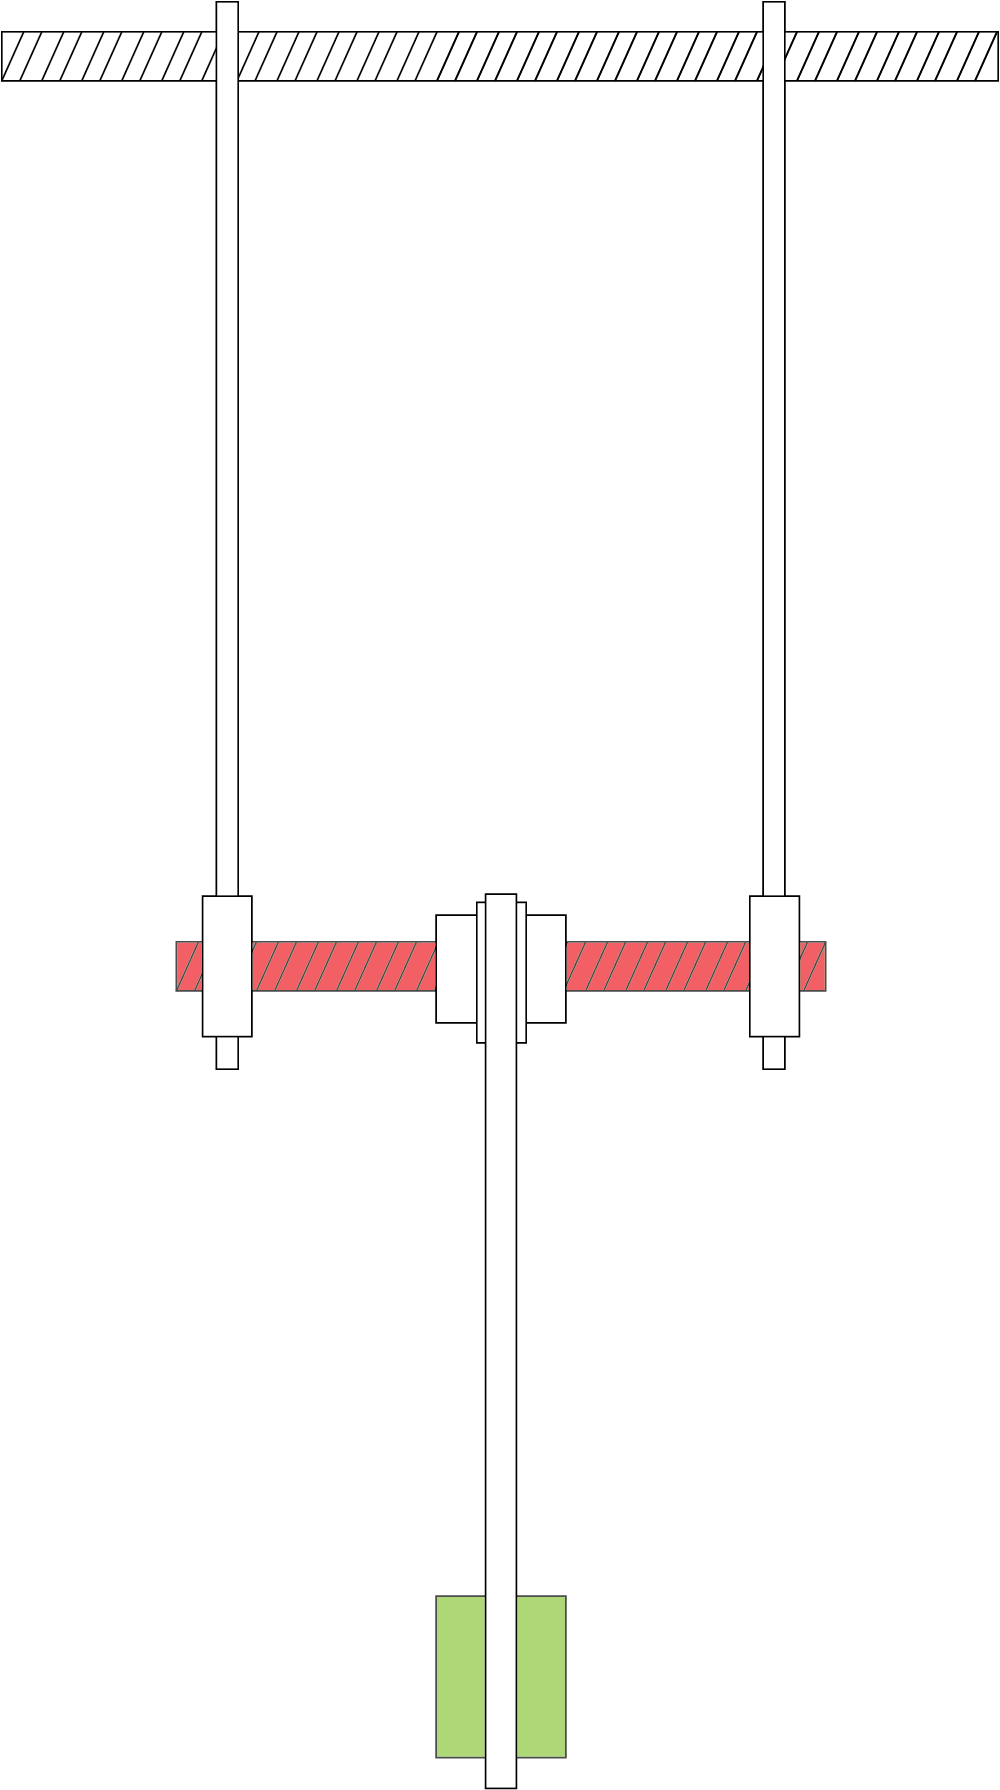
\includegraphics[width=.6\textwidth]{images/pendel-skizze.png}
	\caption{Technische Zeichnung des Pendels}
	\label{pic:skizze_versuchsaufbau}
\end{figure}
\lstset{language=Python}
\lstset{inputencoding=utf8/latin1}
\lstset{numbers=left, numberstyle=\tiny, stepnumber=2, numbersep=5pt}
\lstinputlisting[basicstyle=\footnotesize, label=code1, caption=Implementierung der Simulation in python]{sourceCode/simulation.py}

\begin{center}
\begin{longtable}{lllll}
\caption{Verlauf der Position der beiden Massen über die Zeit des Versuchs. Dabei wird t in s und die Position in m gemessen. (Jeder 10. Messpunkt wird dargestellt.)} \label{xy-table}\\
\hline
\textbf{t} & \textbf{x-Pos. $m_1$} & \textbf{y-Pos $m_1$} & \textbf{x-Pos. $m_2$} & \textbf{y-Pos. $m_2$} \\
\hline
\endfirsthead
\multicolumn{4}{c}%
{\tablename\ \thetable\ -- \textit{Fortsetzung}} \\
\hline
\textbf{t} & \textbf{x-Pos. $m_1$} & \textbf{y-Pos $m_1$} & \textbf{x-Pos. $m_2$} & \textbf{y-Pos. $m_2$} \\
\hline
\endhead
\hline \multicolumn{4}{r}{\textit{Fortsetzung auf der nächsten Seite}} \\
\endfoot
\hline
\endlastfoot
$0.0$&$-0.178$&$-0.237$&$-0.002$&$-0.332$\\
$0.333$&$0.078$&$-0.29$&$0.038$&$-0.475$\\
$0.667$&$0.179$&$-0.242$&$0.031$&$-0.382$\\
$1$&$-0.172$&$-0.242$&$0.018$&$-0.302$\\
$1.334$&$0.106$&$-0.282$&$-0.069$&$-0.359$\\
$1.668$&$0.105$&$-0.282$&$0.143$&$-0.476$\\
$2.002$&$-0.144$&$-0.26$&$0.044$&$-0.326$\\
$2.335$&$0.131$&$-0.271$&$-0.061$&$-0.283$\\
$2.669$&$-0.022$&$-0.299$&$0.074$&$-0.463$\\
$3.003$&$-0.091$&$-0.284$&$0.103$&$-0.315$\\
$3.336$&$0.16$&$-0.255$&$-0.032$&$-0.293$\\
$3.670$&$-0.118$&$-0.273$&$-0.016$&$-0.437$\\
$4.004$&$-0.023$&$-0.298$&$0.14$&$-0.416$\\
$4.337$&$0.175$&$-0.245$&$-0.007$&$-0.329$\\
$4.671$&$-0.166$&$-0.245$&$0.012$&$-0.335$\\
$5.005$&$0.086$&$-0.288$&$-0.023$&$-0.444$\\
$5.338$&$0.155$&$-0.258$&$0.079$&$-0.45$\\
$5.672$&$-0.151$&$-0.256$&$0.033$&$-0.333$\\
$6.006$&$0.12$&$-0.275$&$-0.069$&$-0.312$\\
$6.339$&$-0.014$&$-0.299$&$0.114$&$-0.441$\\
$6.673$&$-0.087$&$-0.285$&$0.095$&$-0.366$\\
$7.007$&$0.139$&$-0.267$&$-0.054$&$-0.292$\\
$7.340$&$-0.125$&$-0.27$&$0.024$&$-0.397$\\
$7.674$&$0.036$&$-0.298$&$0.134$&$-0.473$\\
$8.008$&$0.138$&$-0.268$&$-0.032$&$-0.376$\\
$8.341$&$-0.166$&$-0.246$&$0.014$&$-0.333$\\
$8.675$&$0.144$&$-0.264$&$-0.014$&$-0.378$\\
$9.009$&$0.032$&$-0.298$&$0.13$&$-0.462$\\
$9.342$&$-0.124$&$-0.27$&$0.004$&$-0.428$\\
$9.676$&$0.137$&$-0.267$&$-0.053$&$-0.312$\\
$10.01$&$-0.085$&$-0.286$&$0.104$&$-0.336$\\
$10.34$&$0.046$&$-0.296$&$0.06$&$-0.491$\\
$10.67$&$0.088$&$-0.287$&$-0.089$&$-0.374$\\
$11.01$&$-0.131$&$-0.267$&$0.057$&$-0.334$\\
$11.34$&$0.18$&$-0.24$&$0.032$&$-0.373$\\
$11.67$&$-0.056$&$-0.293$&$0.051$&$-0.452$\\
$12.01$&$-0.091$&$-0.284$&$-0.031$&$-0.478$\\
$12.34$&$0.164$&$-0.252$&$0.012$&$-0.382$\\
$12.67$&$-0.091$&$-0.284$&$0.102$&$-0.311$\\
$13.01$&$0.1$&$-0.283$&$-0.064$&$-0.387$\\
$13.34$&$0.018$&$-0.299$&$-0.037$&$-0.491$\\
$13.68$&$-0.06$&$-0.292$&$0.124$&$-0.364$\\
$14.01$&$0.163$&$-0.253$&$-0.01$&$-0.354$\\
$14.34$&$-0.145$&$-0.259$&$0.014$&$-0.376$\\
$14.68$&$0.087$&$-0.287$&$-0.027$&$-0.44$\\
$15.01$&$0.09$&$-0.286$&$0.107$&$-0.484$\\
$15.34$&$-0.11$&$-0.277$&$0.042$&$-0.407$\\
$15.68$&$0.115$&$-0.277$&$-0.073$&$-0.328$\\
$16.01$&$-0.091$&$-0.284$&$0.088$&$-0.364$\\
$16.34$&$0.103$&$-0.282$&$0.066$&$-0.471$\\
$16.68$&$0.042$&$-0.297$&$-0.061$&$-0.47$\\
$17.01$&$-0.118$&$-0.273$&$0.035$&$-0.404$\\
$17.35$&$0.173$&$-0.245$&$0.019$&$-0.372$\\
$17.68$&$-0.088$&$-0.285$&$0.093$&$-0.357$\\
$18.01$&$0.066$&$-0.292$&$-0.086$&$-0.409$\\
$18.35$&$0.029$&$-0.298$&$0.014$&$-0.495$\\
$18.68$&$-0.043$&$-0.295$&$0.13$&$-0.388$\\
$19.01$&$0.133$&$-0.269$&$-0.038$&$-0.372$\\
$19.35$&$-0.143$&$-0.261$&$0.017$&$-0.378$\\
$19.68$&$0.13$&$-0.271$&$-0.008$&$-0.408$\\
$20.02$&$-0.005$&$-0.298$&$0.123$&$-0.438$\\
$20.35$&$-0.042$&$-0.296$&$-0.019$&$-0.492$\\
$20.68$&$0.092$&$-0.285$&$-0.067$&$-0.403$\\
$21.02$&$-0.076$&$-0.287$&$0.11$&$-0.349$\\

\end{longtable}
\end{center}
